\documentclass{beamer}
\usetheme{metropolis}           % Use metropolis theme
\usepackage{graphicx}
\usepackage{subcaption}
\title{Optimizing a Minimal Language using Pre-trained Language Models}
\date{}
\author{Ajay Narayanan}
\institute{Technical University of Munich}
\begin{document}
  \maketitle

\begin{frame}{Agenda}
	\tableofcontents
\end{frame}

\section{Motivation and Concepts}

% Slide: Why Study Language Optimality?
\begin{frame}{Why Study Language Optimality?}
	\begin{itemize}
		\item Human language evolved for survival and cooperation—not efficiency.
		\item Natural languages are shaped by history, noise, and cognitive constraints.
		\item Can we do better if we start from scratch?
		\item Constructed languages (ConLangs) offer a testing ground.
	\end{itemize}
\end{frame}

% Slide: Trade-offs in Language Design
\begin{frame}{Trade-offs in Language Design}
	\begin{itemize}
		\item Language design faces a trade-off between:
		\begin{itemize}
			\item \textbf{Expressiveness}
			\item \textbf{Efficiency}
		\end{itemize}
		\item Natural languages aren't optimized for either.
		\item Our goal: can we define "optimal" and get closer to it?
	\end{itemize}
\end{frame}

% Slide: Constructed Languages
\begin{frame}{Constructed Languages (ConLangs)}
	\begin{itemize}
		\item ConLangs are intentionally built from first principles.
		\item Vary in purpose: auxiliary, fictional, logical, minimalist, expressive.
		\item We explore how to optimize a ConLang using modern tools.
	\end{itemize}
\end{frame}

% Slide: Role of Language Models
\begin{frame}{Enter Language Models}
	\begin{itemize}
		\item Large Language Models (LLMs) embed knowledge of real languages.
		\item Can they help design new ones?
		\item We use LLMs to:
		\begin{itemize}
			\item Generate and translate language
			\item Analyze simplicity, meaning retention, and structure
		\end{itemize}
	\end{itemize}
\end{frame}

% Slide: Goals
\begin{frame}{Thesis Goals}
	\begin{enumerate}
		\item Define linguistic optimality along measurable axes.
		\item Design a modular pipeline to create efficient ConLangs.
		\item Use LLMs to guide generation, translation, and evaluation.
	\end{enumerate}
\end{frame}

\section{Building the Language Step-by-Step}

% Slide: The Journey Begins
\begin{frame}{The Journey Begins}
	\begin{itemize}
		\item We start with a blank slate.
		\item Step-by-step, we add layers: phonetics → grammar → vocabulary → translation → evaluation.
		\item Each choice is a design decision.
	\end{itemize}
\end{frame}

% Slide: Phonetics
\begin{frame}{Step 1: Choosing Phonemes}
	\begin{itemize}
		\item First, define how words sound: phonemic inventory.
		\item Use the most common phonemes from PHOIBLE.
		\item Simpler inventories → easier learning.
	\end{itemize}
\end{frame}

% Slide: Phonotactics
\begin{frame}{Step 2: Structuring Sounds (Phonotactics)}
	\begin{itemize}
		\item Rules for combining sounds.
		\item We test:
		\begin{itemize}
			\item Basic CV (Consonant-Vowel) structures.
			\item Custom syllable constraints.
		\end{itemize}
	\end{itemize}
\end{frame}

% Slide: Grammar
\begin{frame}{Step 3: Choosing a Grammar}
	\begin{itemize}
		\item What kind of grammar should we use?
		\item Try agglutinative (suffix-based) and isolating (word-order-based).
		\item Implement with reusable grammatical features.
	\end{itemize}
\end{frame}

% Slide: Vocabulary
\begin{frame}{Step 4: Building a Vocabulary}
	\begin{itemize}
		\item Vocabulary = heart of expressiveness.
		\item We test multiple strategies:
		\begin{itemize}
			\item From source
			\item Simplified by clustering
			\item Approximation via embeddings
		\end{itemize}
		\item Trade-off: size vs. meaning retention.
	\end{itemize}
\end{frame}

% Slide: Translation
\begin{frame}{Step 5: Translating Text}
	\begin{itemize}
		\item Use LLMs to translate between English and our ConLang.
		\item Translate and back-translate to test loss of meaning.
		\item Input: paragraphs from known corpora.
	\end{itemize}
\end{frame}

% Slide: Evaluation
\begin{frame}{Step 6: Evaluating Performance}
	\begin{itemize}
		\item We measure:
		\begin{itemize}
			\item Information loss (BLEU, ROUGE, comprehension)
			\item Simplicity (perplexity, vocabulary size, phoneme count)
			\item Zipf's Law compliance
		\end{itemize}
		\item Every pipeline produces scores for comparison.
	\end{itemize}
\end{frame}

% Slide: Tools and Infrastructure
\begin{frame}{Supporting Infrastructure}
	\begin{itemize}
		\item Modular codebase with JSON outputs.
		\item Local + remote LLMs.
		\item Embeddings via MiniLM.
		\item Clustering methods: Agglomerative, KMeans, HDBScan.
	\end{itemize}
\end{frame}

\section{Results and Insights}

% Slide: Phoneme Count
\begin{frame}{Does Phoneme Count Matter?}
	\begin{itemize}
		\item Reducing phoneme count had minimal effect.
		\item Simpler phonology still retained meaning.
	\end{itemize}
	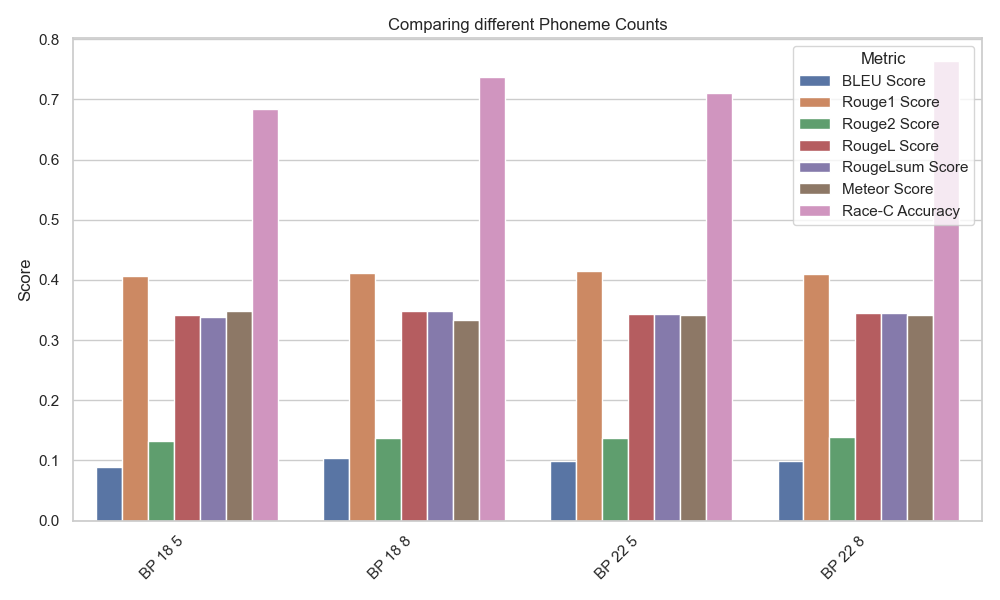
\includegraphics[width=0.7\linewidth]{figures/results/1_effect_of_phoneme_count.png}
\end{frame}

% Slide: Phonotactics
\begin{frame}{Effect of Phonotactics}
	\begin{itemize}
		\item Simplified phonotactics had little impact on comprehension.
		\item Supports minimalist phonological design.
	\end{itemize}
	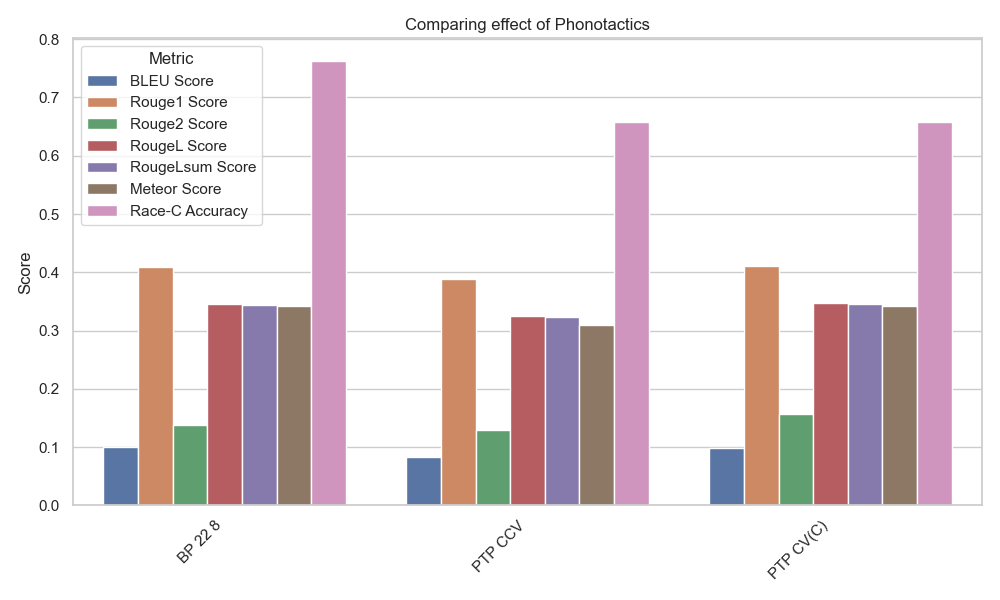
\includegraphics[width=0.7\linewidth]{figures/results/1_effect_of_phonotactics.png}
\end{frame}

% Slide: Grammar
\begin{frame}{Grammar: Agglutinative vs Isolating}
	\begin{itemize}
		\item Translation and comprehension scores were similar.
		\item Only language model perplexity showed differences.
	\end{itemize}
	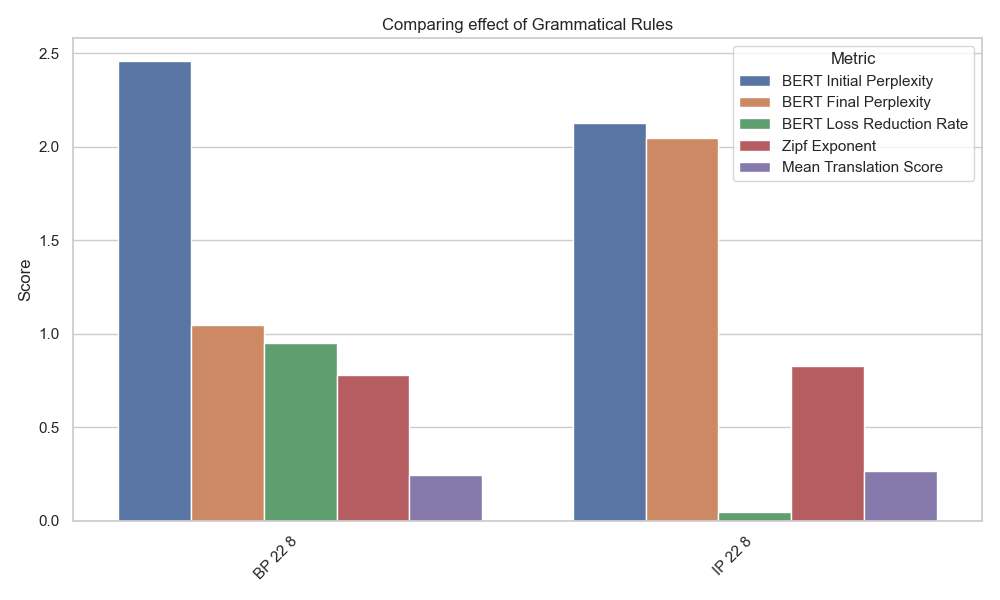
\includegraphics[width=0.7\linewidth]{figures/results/1_effect_of_grammar.png}
\end{frame}

% Slide: Vocabulary Simplification
\begin{frame}{Vocabulary Trade-offs}
	\begin{itemize}
		\item Simplified vocab reduced n-gram translation accuracy.
		\item Meaning-based (Race-C) scores dropped less.
		\item Better score-per-word ratios in simpler methods.
	\end{itemize}
\end{frame}

\begin{frame}{Vocabulary Performance Visuals}
	\begin{columns}
		\column{0.48\textwidth}
		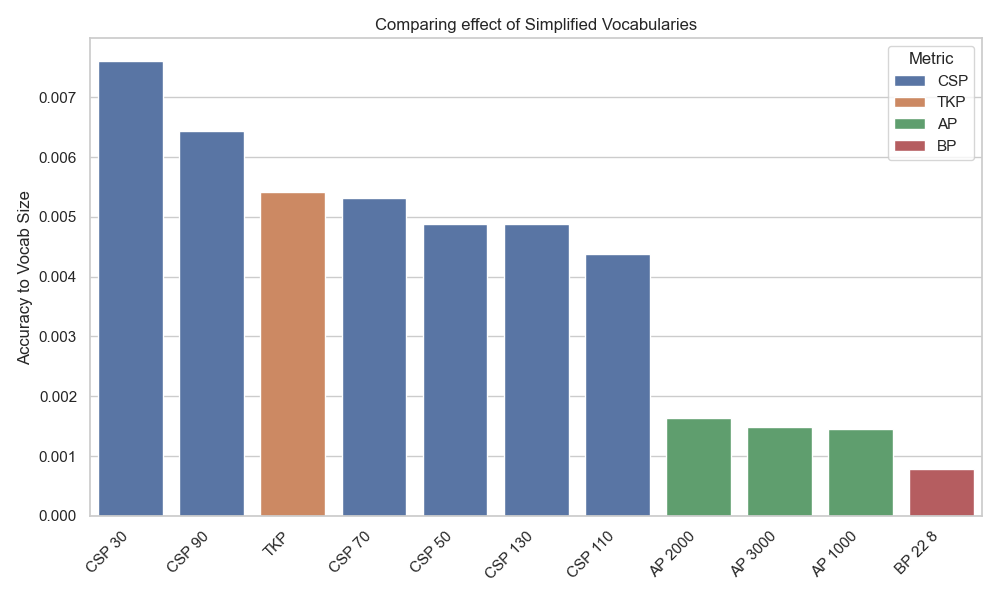
\includegraphics[width=\linewidth]{figures/results/1_effect_of_vocab_simplify.png}
		\captionof{figure}{Race-C Accuracy}
		\column{0.48\textwidth}
		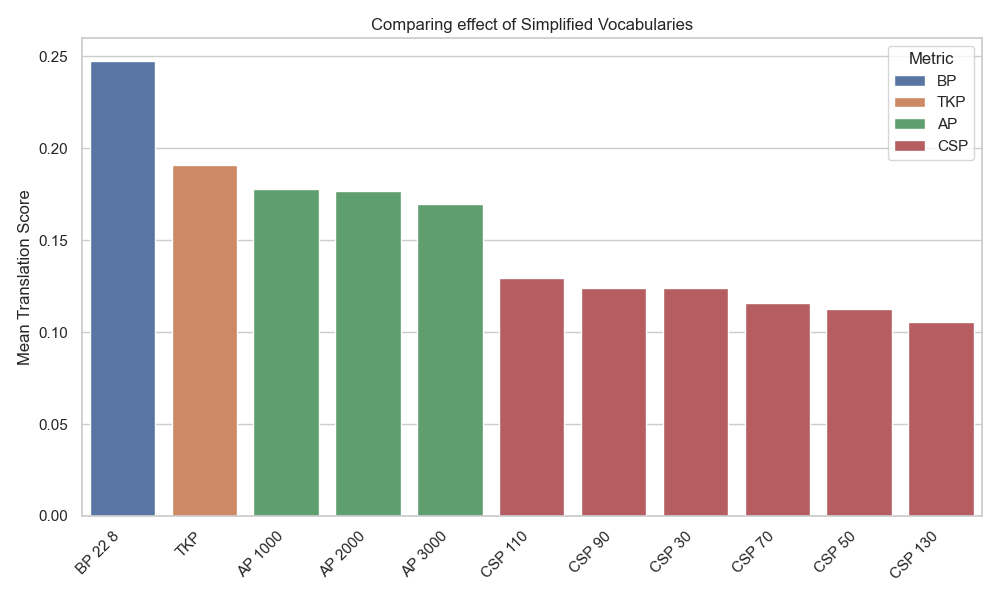
\includegraphics[width=\linewidth]{figures/results/1_effect_of_vocab_simplify_mts.png}
		\captionof{figure}{MTS Score}
	\end{columns}
\end{frame}

% Slide: Temperature
\begin{frame}{Language Model Temperature}
	\begin{itemize}
		\item Higher temperature increases randomness.
		\item Lower values (0.2) more reproducible and stable.
	\end{itemize}
	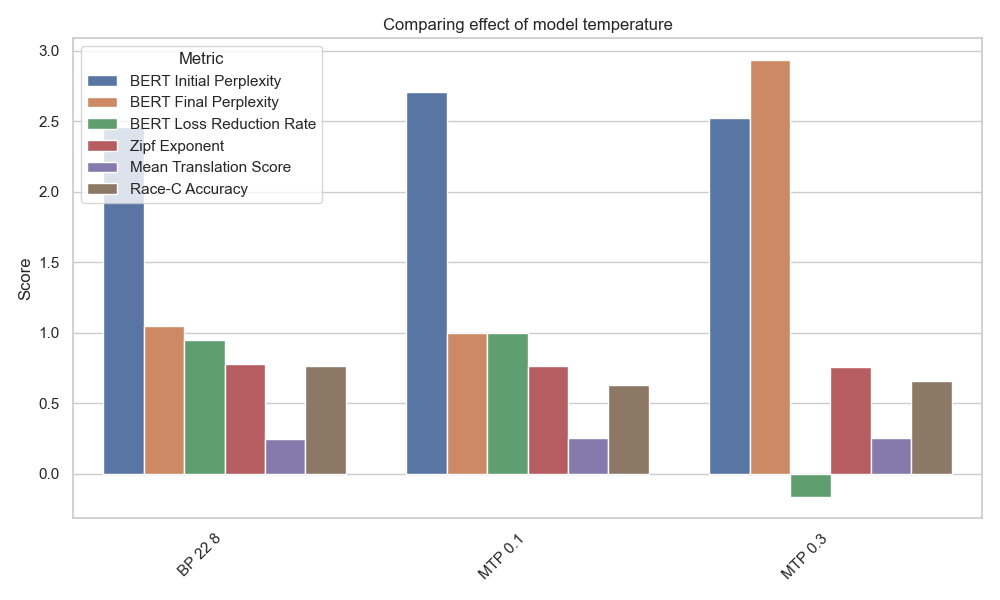
\includegraphics[width=0.7\linewidth]{figures/results/1_effect_of_model_temperature.png}
\end{frame}

% Slide: Comparison Chart
\begin{frame}{Comparing Vocabulary Pipelines}
	\begin{figure}
		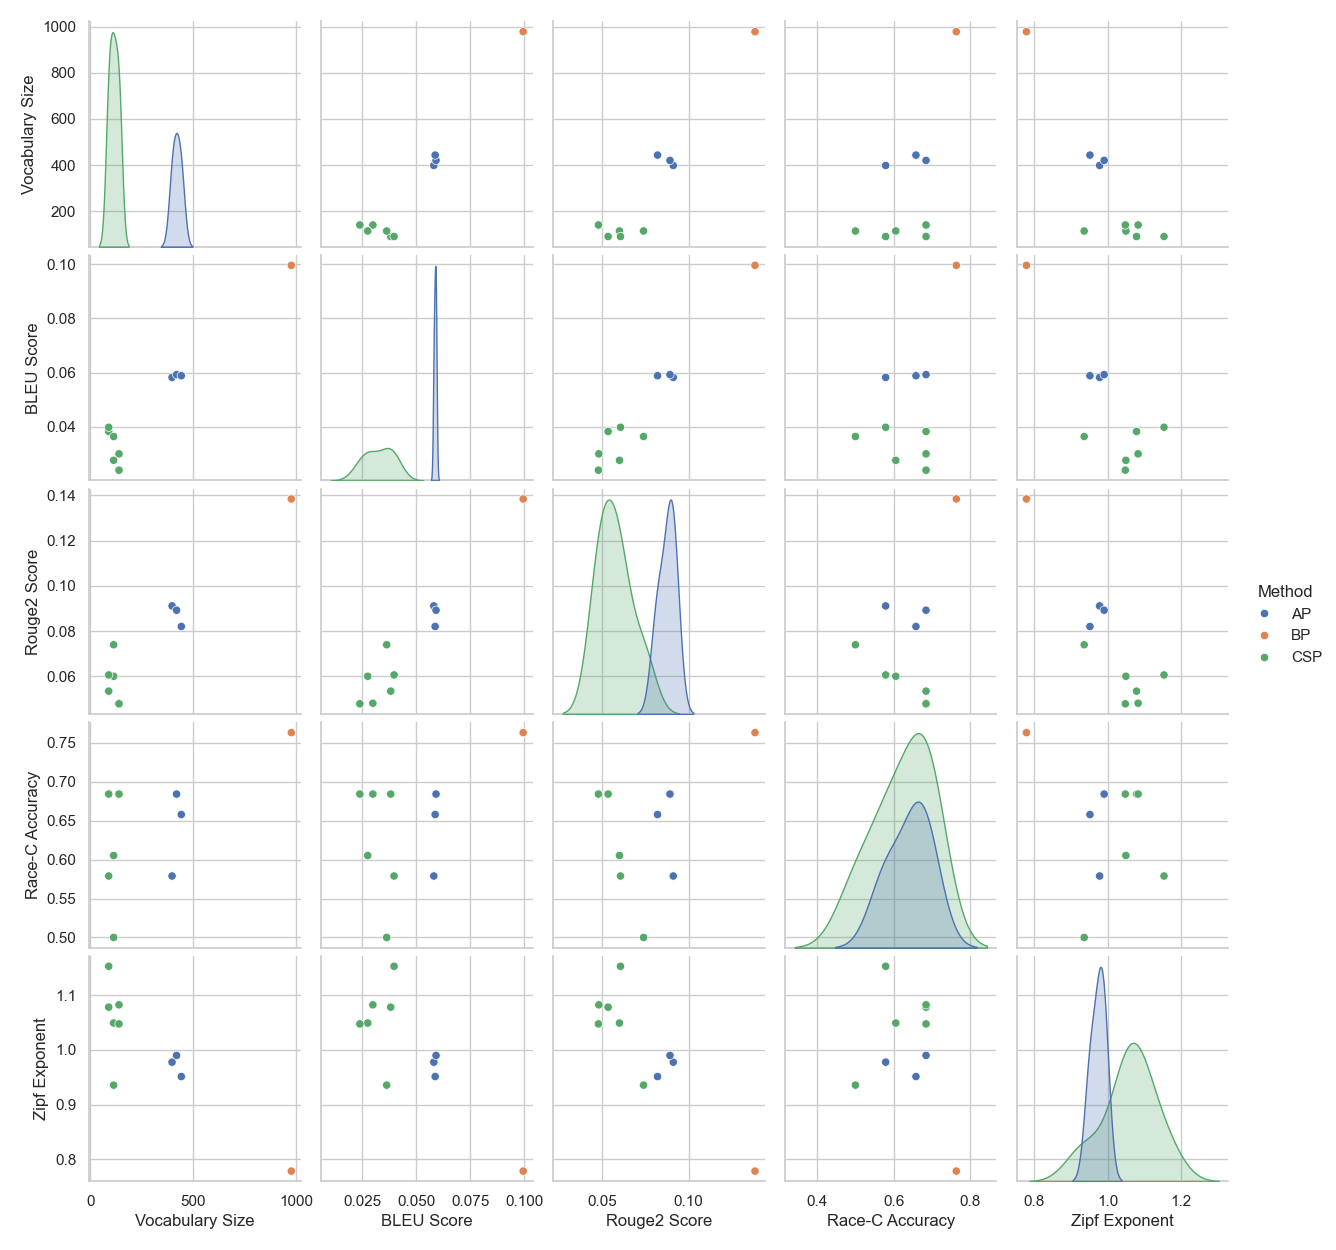
\includegraphics[width=0.7\linewidth]{figures/results/0_pairplot_vocabulary.png}
		\caption{Comparison of different vocabulary generation strategies.}
	\end{figure}
\end{frame}

% Slide: Conclusion
\begin{frame}{Conclusion}
	\begin{itemize}
		\item LLMs can assist in building efficient ConLangs.
		\item Simpler phonology and grammar still retain meaning.
		\item Vocabulary trade-offs are the most sensitive.
		\item Modular pipeline allows repeatable experiments.
	\end{itemize}
\end{frame}

% Slide: Future Work
\begin{frame}{What's Next?}
	\begin{itemize}
		\item Improve vocab generation using semantics.
		\item Evaluate spoken/multimodal ConLangs.
		\item Design user-facing ConLang creators.
		\item Explore LLM co-evolution with constructed languages.
	\end{itemize}
\end{frame}

% Slide: Thank You
\begin{frame}{Questions?}
	\centering
	Thank you!\\
	Questions are welcome.
\end{frame}

\end{document}